\documentclass{beamer}

% There are many different themes available for Beamer. A comprehensive
% list with examples is given here:
% http://deic.uab.es/~iblanes/beamer_gallery/index_by_theme.html
% You can uncomment the themes below if you would like to use a different
% one:
%\usetheme{AnnArbor}
%\usetheme{Antibes}
%\usetheme{Bergen}
%\usetheme{Berkeley}
%\usetheme{Berlin}
%\usetheme{Boadilla}
%\usetheme{boxes}
%\usetheme{CambridgeUS}
%\usetheme{Copenhagen}
%\usetheme{Darmstadt}
%\usetheme{default}
%\usetheme{Frankfurt}
%\usetheme{Goettingen}
%\usetheme{Hannover}
%\usetheme{Ilmenau}
%\usetheme{JuanLesPins}
%\usetheme{Luebeck}
\usetheme{Madrid}
%\usetheme{Malmoe}
%\usetheme{Marburg}
%\usetheme{Montpellier}
%\usetheme{PaloAlto}
%\usetheme{Pittsburgh}
%\usetheme{Rochester}
%\usetheme{Singapore}
%\usetheme{Szeged}
%\usetheme{Warsaw}

\title{Parallel Programming Mini Project 01}

% A subtitle is optional and this may be deleted
\subtitle{Simulation of Stock Prices using Geometric Brownian Motion}

\author{Gaurav Tolani(201352021)\inst{} \and Akhilesh Kumar(201351009)}
% - Give the names in the same order as the appear in the paper.
% - Use the \inst{?} command only if the authors have different
%   affiliation.

\institute[IIITV] % (optional, but mostly needed)
{
  \inst{}%
  Indian Institute of Information Technology, Vadodara\\
  
  }
% - Use the \inst command only if there are several affiliations.
% - Keep it simple, no one is interested in your street address.

\date{September, 2016}
% - Either use conference name or its abbreviation.
% - Not really informative to the audience, more for people (including
%   yourself) who are reading the slides online

\subject{Theoretical Computer Science}
% This is only inserted into the PDF information catalog. Can be left
% out. 

% If you have a file called "university-logo-filename.xxx", where xxx
% is a graphic format that can be processed by latex or pdflatex,
% resp., then you can add a logo as follows:
 \pgfdeclareimage[height=0.8cm]{university-logo}{logo_iiitv.png}
 \logo{\pgfuseimage{university-logo}}

% Delete this, if you do not want the table of contents to pop up at
% the beginning of each subsection:
\AtBeginSubsection[]
{
  \begin{frame}<beamer>{Outline}
    \tableofcontents[currentsection,currentsubsection]
  \end{frame}
}

% Let's get started
\begin{document}

\begin{frame}
  \titlepage
\end{frame}

\begin{frame}{Outline}
  \tableofcontents
  % You might wish to add the option [pausesections]
\end{frame}

% Section and subsections will appear in the presentation overview
% and table of contents.
\section{Problem}

\subsection{Problem Statement}

\begin{frame}{Problem Statement}
  \begin{itemize}
  \item {
    Doing stock prices simulation using Geometric Brownian Motion and comparing the efficiency and time of different algorithms and langauges for a number of simulations.
  }
  \end{itemize}
\end{frame}

\subsection{Brownian Movement}

\begin{frame}{Brownian Movement}
  \begin{itemize}
  \item {
    Brownian motion is the random motion of particles suspended in a
fluid (a liquid or a gas) resulting from their collision with the fast-
moving atoms or molecules in the gas or liquid.
  }
  
  \end{itemize}
\end{frame}

\subsection{Geometric Brownian Motion}

\begin{frame}{Geometric Brownian Motion}
  \begin{figure}
  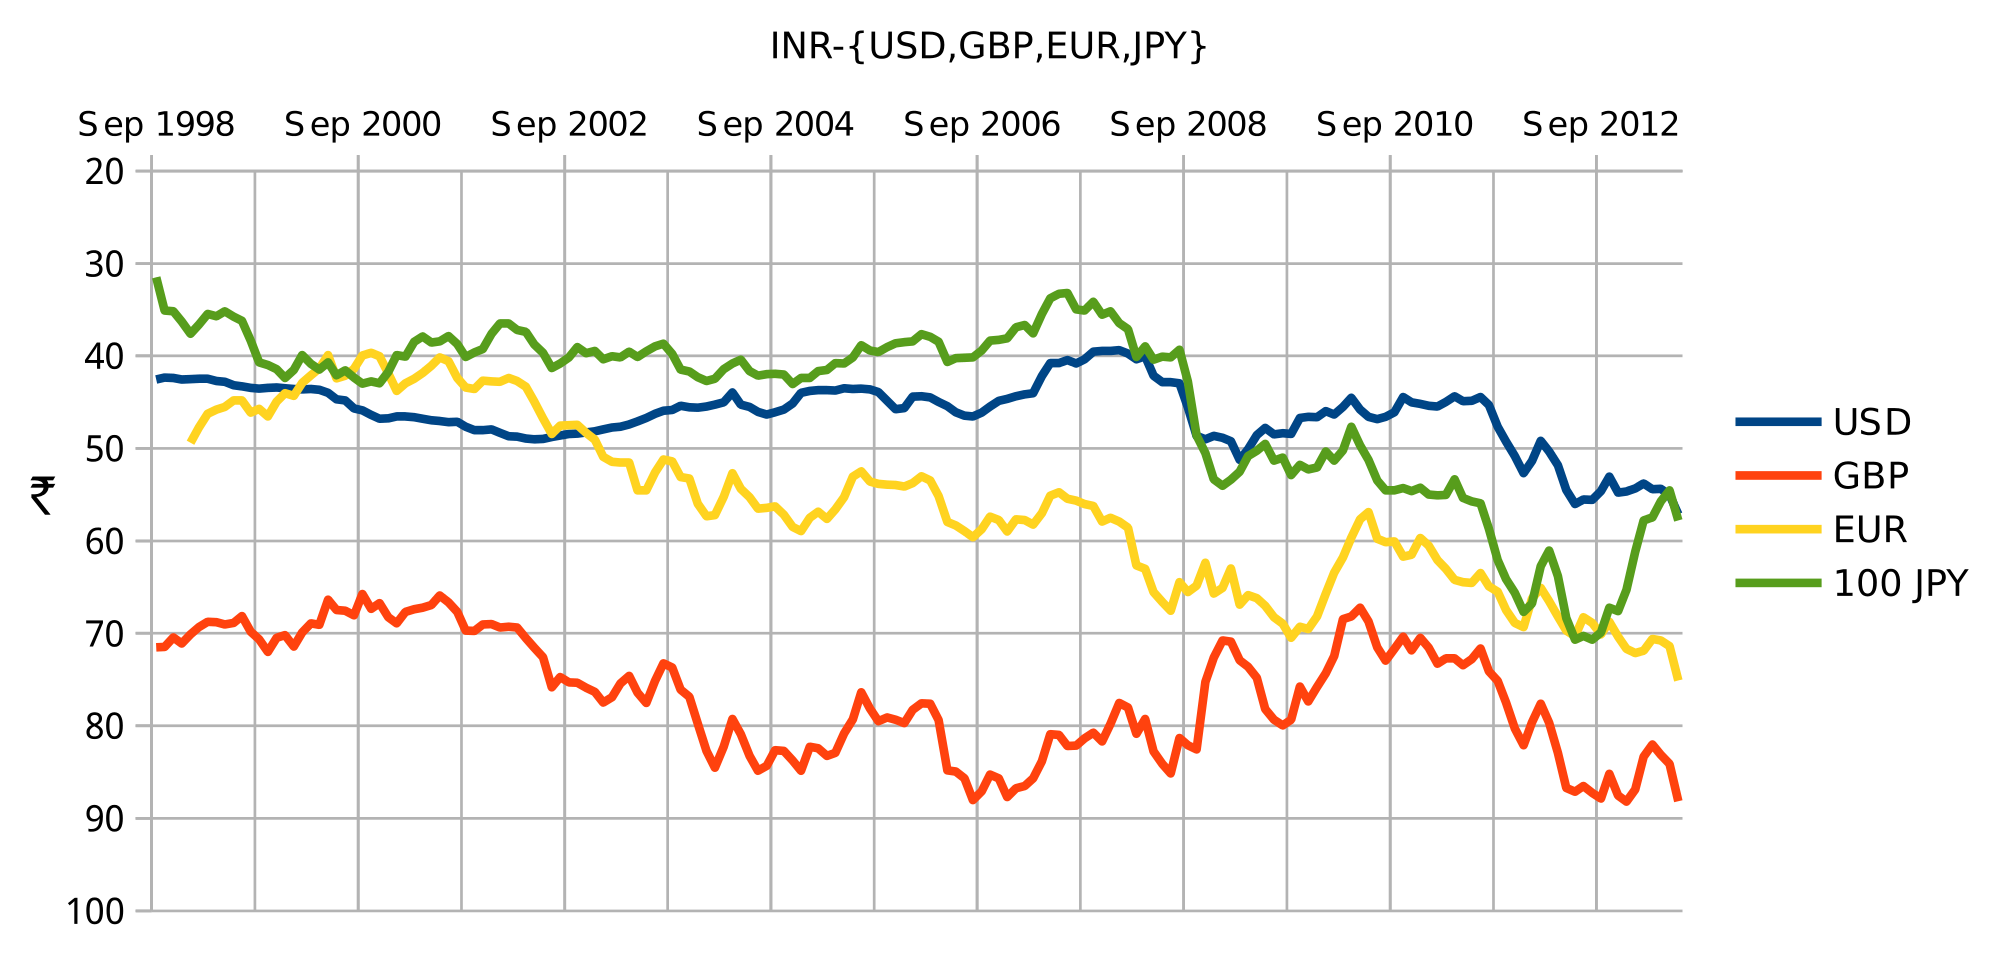
\includegraphics[width=10cm,height=5cm]{Brownian_Motion}\\
  \end{figure}
  \begin{itemize}
  
  \item {
    What? Simple Continuous time stochastic(probabilistic) processes.
  }
  \item {
    Why? Mostly to generate and simulate large amount of random data.
  }
  \item {
     Then Monte Carlo simulations are used to predict the future data many times over.
  }

  \end{itemize}
\end{frame}

\subsection{Financial Modeling}

% You can reveal the parts of a slide one at a time
% with the \pause command:
\begin{frame}{Stock Prices Simulation}
  \begin{itemize}
  \item{
    Geometric Brownian Motion is used to generate random data over a number of stock prices. 
  }
  \item {   
    Given: Initial Stock Price \\
           \hspace{11mm}\small{{\%}} Increment in Prices Required\\
           \hspace{11mm}\small{{\%}} Variance\\
           \hspace{11mm}Time\\
           \hspace{11mm}Number of simulations\\
  }
  \item{
       $S_{t}=S_{0} \times e^{\mu_{t} + \sigma_{t} z}$ \\
       $S_{t}$ is the Price of Stock at time T \\        
       $S_{0}$ is the Initial Price of Stock \\
       ${\mu}$ and ${\sigma}$ are the drift and volatility parameter respectively.\\
  }
  % You can also specify when the content should appear
  % by using <n->:
  % or you can use the \uncover command to reveal general
  % content (not just \items):
  \end{itemize}
\end{frame}
\section{Serial Code}

\subsection{Algorithm}

\begin{frame}{Algorithm}{}
An algorithm for simulating the stock price at time t$>$0, given that current price at time t=0 is $S_{0}$ is as follows:\\
  
  \begin{itemize}
   
  \item {
    Generate random variable z $\sim$ N(0,1)
    
  }
  \item {
    Set $\mu_{t}=(\mu - \sigma^{2}/2)t$ and $\sigma_{t}=\sigma t^{0.5}$
  }
  \item {
  Set $S_{t}=S_{0} \times e^{\mu_{t} + \sigma_{t} z}$
   }
  \end{itemize}
\end{frame}

\subsection{Output Snapshots}

\begin{frame}{Output Snapshots for 'R' and 'C'}{}
\begin{figure}
\begin{columns}[t]
\column{.5\textwidth}

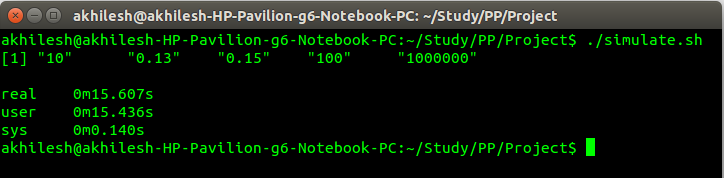
\includegraphics[width=6cm,height=5cm]{1000000}\\

\column{.5\textwidth}

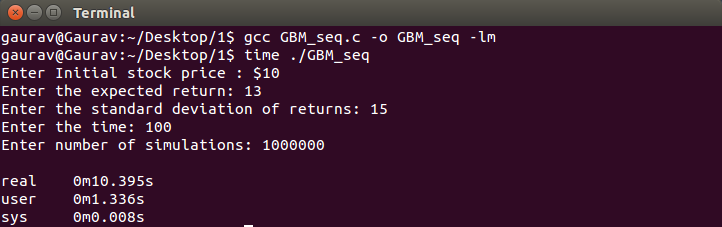
\includegraphics[width=6cm,height=5cm]{1000000_GBM_SERIAL}\\

\end{columns}

\caption{Brownian motion graph for 1000000 simulations}

\end{figure}
  
\end{frame}



\subsection{Graphs}
\begin{frame}{Graphs}{}

\begin{figure}
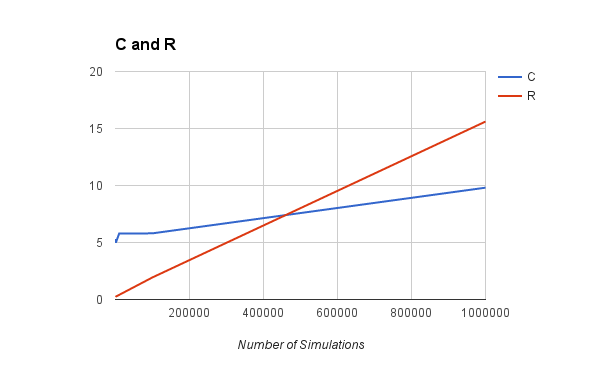
\includegraphics[width=10cm,height=6cm]{CvsR}\\
\caption{Graph Between 'C' and 'R' for different number of simulations}

\end{figure}

\end{frame}

\subsection{Memory Usage}

\begin{frame}{Output Snapshots for 'R' and 'C'}{}
\begin{figure}
\begin{columns}[t]
\column{.5\textwidth}

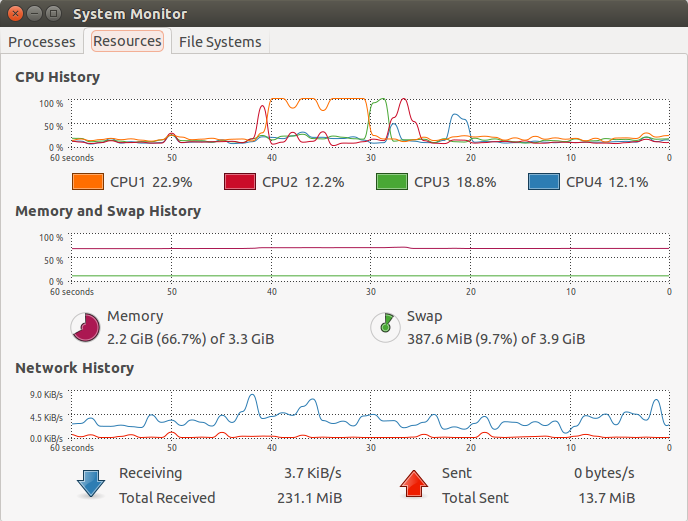
\includegraphics[width=6cm,height=5cm]{1000000_sys_mon}\\

\column{.5\textwidth}

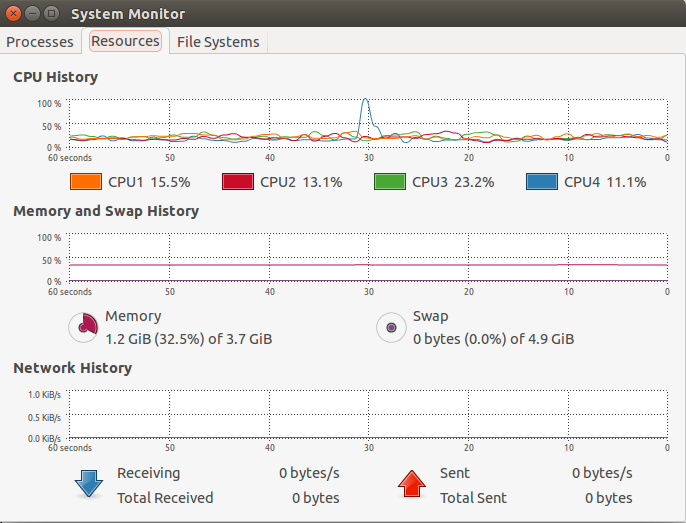
\includegraphics[width=6cm,height=5cm]{CPU_usage_GBM_seq}\\

\end{columns}

\caption{System Monitor(CPU Usage) for 1000000 simulations}

\end{figure}
  
\end{frame}


\section{Conclusion}
\subsection{Conclusion}
\begin{frame}{conclusion}{}
  \begin{itemize}
  \item {
    With Increasing Number of Simulations, Execution time Increases
  }
  \item {
   Time for 1000000 simulations is double in case of 'C' and approx. 14 times in 'R' as compared to 100000 simulations
   }
  \item {
    CPU usage is not at full efficiency in any of the cases which is not the ideal condition.
  }
  \item {
   It is most probable that parallelizing the code will increase the performance of the algorithm.
  }
    
  \end{itemize}
    
\end{frame}


% Placing a * after \section means it will not show in the
% outline or table of contents.


\begin{frame}{}{}
\begin{center}
\Huge Thank You
\end{center}
\end{frame}


% All of the following is optional and typically not needed. 

\end{document}


